\subsection{Camera Estimation}
\seclabel{nrsfm}
We use the framework of \nrsfm \cite{Bregler2000} to jointly estimate the projection parameters (rotation, translation and scale) for all training instances in each class. Originally proposed for recovering shape and deformations from video \cite{nrsfm_priors,Torresani2008NRSFM,varnrsfm2013,Bregler2000}, NRSfM is a natural choice for camera estimation from sparse correspondences as intra-class variation may become a confounding factor if not modeled explicitly. However, the performance of such algorithms has only been explored on simple categories, such as SUV's \cite{Zhu_ModelEvolution:2010} or flower petal and clown fish \cite{prasad2010finding}. Closer to our work, Hejrati and Ramanan \cite{HejratiR12} used NRSfM on a larger class (cars) but need a predictive detector to fill-in missing data (occluded keypoints) which we do not assume to have here.

%To cope with the highly under-constrained nature of the problem most methods have dwelled on low-rank factorizations of the shape matrix \cite{Bregler2000,Brand2005}, or on imposing priors on shapes and deformations \cite{Torresani2008NRSFM,nrsfm_priors,varnrsfm2013}. }

We closely follow the EM-PPCA formulation of Torresani \etal\cite{Torresani2008NRSFM} and propose a simple extension to the algorithm that incorporates silhouette information in addition to keypoint correspondences to robustly recover cameras and shape bases. Energies similar to ours have been proposed in the shape-from-silhouette  \cite{balloonshapes} and rigid structure-from-motion \cite{carvi14} literature but, to the best of our knowledge, not in conjunction with NRSfM.

\paragraph{NRSfM Model Formulation.} We are provided with an annotated training set $T:\{(O_n, P_n)\}_{n=1}^N$, where $O_n$ is the instance silhouette and $P_n \in \mathbb{R}^{2 \times K}$ denotes the annotated keypoint coordinates, possibly with missing entries (occluded/truncated keypoints). The annotated keypoints $P_n$ are  projections of the underlying 3D points $W_n \in \mathbb{R}^{3 \times K}$ via the projection function $\pi_n$. In the \nrsfm model, the space of 3D keypoint locations $W_n$ is parametrized linearly and the projection function is assumed to be weakly orthographic \ie $\pi_n \equiv (c_n, R_n, T_n)$, where $c_n$ represents scale, $R_n \in \mathbb{R}^{2 \times 3}$ denotes rotation and $T_n \in \mathbb{R}^{1 \times 2}$ corresponds to 2D translation. Our goal is to infer the camera parameters $(c_n, R_n, T_n)$ as well as 3D keypoint locations $W_n$ for all instances in the annotated training set.

Formally, our adaptation of the \nrsfm algorithm in \cite{Torresani2008NRSFM} corresponds to maximizing the likelihood of the following model:

\begin{equation}
\begin{aligned}
&{P_{n}} = c_nR_nW_{n} + 1^TT_{n} + N_{n}\\
&W_n = \bar{W} + \sum\limits_{k=1}^B U_b z_{nb} \\
&z_n \sim \mathcal{N}(0,I), \quad N^k_{n}\sim \mathcal{N}(0,\sigma^2 I)
\end{aligned}
\end{equation}
\begin{align}
\text{subject to:}\nonumber &\quad R_nR_{n}^{T} = I_2 \\
\eqlabel{sil_constraint}
\sum\limits_{k=1}^K C_{n}^{mask}(p_{k,n}) &= 0, \quad \forall n\in \{1,\cdots,N\}
\end{align}

Here, the (partially) observed keypoint locations $P_n$ are assumed to be the projection under $\pi_n \equiv (c_n, R_n, T_n)$ of the 3D shape $W_n$ with white noise $N_n$. The shape is parameterized as a factored Gaussian with a mean shape $\bar{W}$, $B$ basis vectors $[U_1,U_2, \cdots,U_B] = U$ and latent deformation parameters $z_n$. Our key modification is constraint in \eqref{sil_constraint} where $C_{n}^{mask}$ denotes the Chamfer distance field of the $n^{th}$ instance's binary mask and says that all keypoints $p_{k,n}$ of instance $n$ should lie inside its binary mask. We observed that this results in more accurate cameras as well as more meaningful shape bases learnt from the data.

\paragraph{Learning.} The likelihood of the above model is maximized using the EM algorithm. Missing data (occluded keypoints) is dealt with by ``filling-in" the values using the forward equations after the E-step. The algorithm computes shape parameters $\{\bar{W},U\}$, rigid body transformations $\{c_n,R_n,T_n\}$ as well as the deformation parameters $\{z_n\}$ for each training instance $n$. In practice, we augment the data using horizontally mirrored images to exploit bilateral symmetry in the object classes considered. We also precompute the Chamfer distance fields for the whole set to speed up computation. As shown in \figref{nrsfm_images}, \nrsfm  allows us to reliably predict cameras while being robust to intraclass variations.

\begin{figure}[htb!]
  \centering
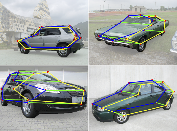
\includegraphics[width=.8\linewidth]{figures/categoryshapes/NRSFMCars.pdf}
\caption{NRSfM camera estimation: Estimated cameras visualized using a 3D car wireframe.}
\figlabel{nrsfm_images}
\end{figure}
